\begin{figure}[h]
    \centering
    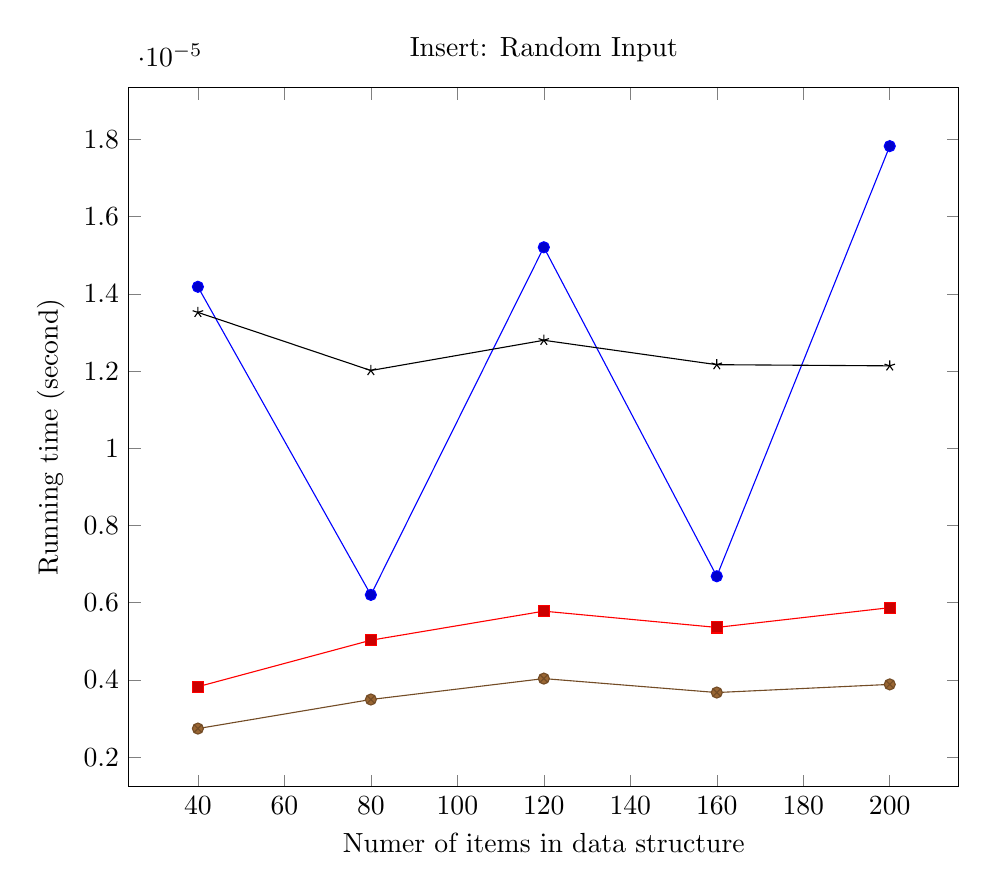
\begin{tikzpicture}
        \begin{axis}[
            xlabel={Numer of items in data structure},
            ylabel={Running time (second)},
            title={Insert: Random Input},
            width=\textwidth
        ]
		\addplot coordinates {
			(200, 1.782957993569645e-05)
			(160, 6.68609247588825e-06)
			(120, 1.5209354505957284e-05)
			(80, 6.2042119370830925e-06)
			(40, 1.4185358361001876e-05)
		};
		\addplot coordinates {
			(200, 5.872919066657323e-06)
			(160, 5.360920994179619e-06)
			(120, 5.782566465634131e-06)
			(80, 5.029628123753849e-06)
			(40, 3.824926776746506e-06)
		};
		\addplot coordinates {
			(200, 3.885161844097151e-06)
			(160, 3.6743391083726705e-06)
			(120, 4.035749512470988e-06)
			(80, 3.4936339063207365e-06)
			(40, 2.740695564440454e-06)
		};
		\addplot coordinates {
			(200, 1.213736607109106e-05)
			(160, 1.2167483604769158e-05)
			(120, 1.2799951811948152e-05)
			(80, 1.2016895936395323e-05)
			(40, 1.3522772620150336e-05)
		};
        \legend{}
        \end{axis}
    \end{tikzpicture}
    \caption{Average of 0 operations, benchmarked every 0, starting at 0.}
\end{figure}